\documentclass[instructions]{uqthesis}
%\documentclass[final]{uqthesis} 


%*************************************
% FOR YOUR FINAL THESIS
%*************************************

%IMPORTANT! 
%The default document class (above - line 1 & 2) for the template is \documentclass[instructions]{uqthesis} - this document class will show instructional material and examples relevant to the preliminary material in the compiled PDF preview. THESE INSTRUCTIONS ARE FOR YOUR REFERENCE ONLY AND ARE NOT TO BE INCLUDED IN YOUR FINAL THESIS! 

%To turn off these instructions in your final thesis you MUST use the document class \documentclass[final]{uqthesis} 
%To activate the final thesis document class you must UN-COMMENT THIS DOCUMENT CLASS (remove the % from the start of line 2) and comment out the instructional document class on line 1 (add % to the start of line 1). 


\input{LaTexPackages.tex}

% ***************************************************
% Title page
% ***************************************************
%***THESIS TITLE***
%Use Sentence Case (capitalise only the first word and proper nouns).

\title{FPGA packet filter with Ethernet MAC and web server using a RISC-V softcore processor }
\subtitle{Thesis}

\author{Matthew Gilpin}
\studentnumber{45801600}



\date{Semester 1, 2023}
\submittedfor{Thesis - REIT4841}


\school{School of Electrical Engineering and Computer Science}



\date{2023}



\begin{document}

\frontmatter
% Assemble title page
\maketitle
\clearpage

% ***************************************************
% Preface
%****************************************************
\section{Abstract}
\normalfont
%Open abstract.tex to edit
% ***************************************************
% Abstract
% ***************************************************
% TO PRODUCE A STAND-ALONE PDF OF YOUR ABSTRACT, uncomment this section and the \end{document} at the end of the file by removing the % from the start of each line.

%\documentclass[12pt, a4paper]{memoir}

%\input{LaTexPackages.tex}

%\begin{document}

%\begin{center}
	%\textbf{\large Your title goes here}

	%\textbf{Abstract}

	%Your Name, The University of Queensland, 20??
%\end{center}


This thesis presents the design and implementation of both a hardware Ethernet Media Access Control (MAC) and packet filter on a Xilinx Artix 7 100T FPGA, specifically with the Digilent Artix 7 FPGA development board which includes a Reduced Media-Independent Interface (RMII) physical (PHY) interface chip. The primary objective of this work was to implement a firewall to improve security in the embedded systems space and to then host a web server on an onboard RISC-V softcore for configuration. More specifically, a NEORV32 RISC-V System on Chip (SoC) was used to interface the hardware over a Wishbone bus with the software hosting the webserver with FreeRTOS utilising both the Freertos-Plus-TCP and FreeRTPS-Plus-FAT libraries. 

The wirespeed hardware five-tuple packet filter, analysing the destination IP, source IP, destination port, source port and protocol, showcased an added delay of just $4\mu s$ irrespective of packet lengths while potentially enhancing security over software based implementations. Many performance benchmarks were also conducted and concluded in a relative power draw of 0.51W including the microprocessor. In comparison other platforms such as the Nucleo-F767ZI, Raspberry Pi Pico with WIZ5500 and MilkV-Duo were evaluated for their performance and efficiency.  

In addition, the web server hosted a static single page application style website using Vue.js and Tailwindcss which was all stored on a microSD card and accessed over the SPI interface and using the FAT32 filesystem. UDP round trip times were also measured for all platforms resulting in an average delay of 1.45ms for the FPGA board which included an added 1ms delay. 

Although effective, the packet classifier lacks support for IPv6 and only is applied to incoming traffic, while the firmware forgoes support for HTTPS. Given the FPGA's resource consumption of 11,738 slice LUTs and 12,505 slice registers, potential optimisations are discussed to overcome these shortcomings. A recommendation for future designs includes incorporating the efficiency and performance of the MilkV Duo RISC-V (CVITEK CV1800B based) board with an integrated hardware packet filter for a fast and secure embedded system platform. 

%\end{document}

\clearpage
% ***************************************************
\section*{Declaration by author}
%DO NOT EDIT.
\input{./Authordeclaration.tex}

\clearpage
%YOU MUST EDIT THIS DOCUMENT.
% ***************************************************
% PRELIMINARY PAGES
% ***************************************************
% The instructions contained within this part of the thesis template need to be suppressed from the final thesis. There are instructions on how to do this in the MainThesis.tex file.

% To ensure your work is not suppressed with the instructions please add your text only where instructed.


\clearpage
\pagestyle{headings}


%***Table of Contents***
%These generate the table of contents, list of figures, and list of tables from items tagged with a \label{} command.
\tableofcontents
	\clearpage
\listoffigures
\listoftables

% \input{./PreliminaryAndBackPages/Symbols.tex} %List of symbols. REMOVE IF NOT NEEDED.

%***End of front matter***

% ***************************************************
% Thesis Content
%****************************************************
\mainmatter

%Each chapter is a separate .tex file. Use \input to load them here, as demonstrated below for Chapter 1 and Chapter 2.
%We recommend keeping each in a separate subfolder, with its accompanying figures, etc. This is how the template is currently structured.
%If you wish to divide your thesis into parts (each containing multiple chapters), us the \part{} command.

%CHAPTER 1
\chapter[Introduction]{Introduction}
\label{Chap:Intro}

% ***************************************************
% Introduction
% ***************************************************



This chapter provides the necessary background and reasoning behind the proposed project. 

\section{Background }
In a technology age of growing numbers of cyber attacks and growing number of Internet-of-Things (IoT) devices being interconnected, it's 
paramount to ensure these devices operate safetly and securely. 

\section{Topic}

% ********* Enter your text below this line: ********

There are a plethora of different ways to reduce the likelyhood of cyber attacks.
A common approach is to employ a firewall to filter out potentially malicious packets. 

This project focuses primarily on securing edge IoT Ethernet networks. 


\section{Aims}

The aims of the proposed FPGA Ethernet controller and web interface on a RISC-V processor are:

\begin{itemize}
    \item Increase security to edge IoT networks.
    \item Increase the power efficiency for wire-speed firewalls.
\end{itemize}




%CHAPTER 2
\chapter[Literature review]{Literature review }
\label{Chap:label}	%CREATE YOUR OWN LABEL.
\pagestyle{headings}



Some of the concepts behind the proposed project, such as an Ethernet MAC or RISC-V processor are not new. Consequently, there is a variety of previous work 
in these areas. This part of the proposal will explore the prior work related to the project. 


\section{Field Programmable Gate Arrays}
\label{subsection:fpga}	
First introduced by Xilinx in 1984, field programmable gate arrays (FPGAs) allowed for large custom logic designs to be recognised without the need for 
expensive application specific integrated circuits (ASICs). More importantly, FPGAs did not suffer from the same scalability issues that
programmable array logic (PAL) encountered and has allowed for larger and more complex designs \cite{30YearsOfFPGA}. 

A big advantage to custom logic is the ability to create highly parallelised designs with lower latencies than software based serialised algorithms. This comes down to 
having a great degree of freedom when it comes to designing the architecture and ability to optimise for specific tasks.
As such, FPGAs have became ubiquitous in both digital signal processing and for accelerating an assortment of heterogeneous computing architectures and processes \cite{FPGAComputing}.
System on chip (SoC) design with custom hardware acceleration modules is an active area research. As \cite{FPGAComputing} points out, there is a focus towards 
using both hardware and software in \textit{edge} devices due to growing numbers of IoT devices.


Several papers, \cite{LwIPFPGAFirewall} \cite{IPFPGAFirewall2000} \cite{packetFilteringFPGA}, have proposed a range of other related FPGA based firewalls that have 
different properties and focus on different optimisations. The key benefit to these firewalls is their high performance - namely, low latency, and high throughput. 
Article \cite{LwIPFPGAFirewall} proposed an Ethernet firewall using LwIP (A TCP/IP stack) with five-tuple binding (the five filtered parameters in packet filters) 
to achieve a throughput of 950Mbps with a latency of 61.266us. A conference proceeding in 2000 \cite{IPFPGAFirewall2000} used a comparator unit to check the 
fields of the IP headers obtained a filtering rate of 500,000 packets per second. 


The enabling concept behind the above FPGA based firewalls is SoC design which involves integrating multiple components into a single package, or in this case a 
single FPGA. Often these will include small softcore microprocessors and some custom hardware such as the Ethernet or packet filtering like the proposed packet filters in \cite{LwIPFPGAFirewall}.
Having a microprocessor in the FPGA design can significantly reduce the complexity of the design and allows for quick and easy development in software instead of 
hardware \cite{SoftcoreBasedEmbeddedSystems}. In FPGA design, softcore processors are configurable and can be modelled in a hardware description language (HDL) 
which can then be synthesised onto ASICs or FPGAs hardware \cite{SoftcoreBasedEmbeddedSystems}. There are several softcore processors available for FPGA 
designs including ARM Cortex, Nios II, MicroBlaze, and RISC-V. 
 
While recently the royalty free RISC-V based cores have been popular amongst many SoC designs, other older processors are still common in the literature. The two 
big FPGA vendors, Xilinx (now AMD) and Altera (now Intel) have their own RISC based softcores. As an example, Janik et al. \cite{LwIPMicroblaze} used Xilinx's MicroBlaze processor 
as a media converter between optical (SFP interface) and copper (Ethernet) networks. Likewise, Altera's Nios II can be found in a variety of research papers 
including an embedded web server which significantly simplified the design \cite{NiosIIWebserver}. 



\section{Packet Filter Firewall}

Usually, the first line of defence against bad actors, firewalls play a vital component in computer networks and as such can become vastly complex. 
In essence, the job of a firewall is to isolate and restrict access to an internal network from an external one to increase security \cite{BuildingInternetFirewalls}.

There are several types of firewalls such as packet filters (PF), stateful packet firewalls and application firewalls \cite{FirewallsBook}. 
Traditional PFs are considered as stateless and filter exclusively on the fields in the network (layer 2) and transport 
(layer 3) layer headers \cite{FirewallsBook}. Such fields include IP addresses, port numbers and protocol type.

Due to this, PFs are inherently simple and efficient. Consequently, they are widely available and can be either implemented in software or in 
hardware \cite{BuildingInternetFirewalls}. The book, \cite{BuildingInternetFirewalls}, also highlights some inherent flaws with PFs which include not being able 
to suppress sophisticated attacks and in some cases, can be challenging to properly configure. More advanced firewalls can perform deep packet inspection which 
explore the contents of the higher layers to better evaluate a packets true intention \cite{FirewallsBook}. 

While firewalls such as \textit{iptables} in Linux are software based, hardware acceleration can vastly improve the performance of a packet filter. As stated in section 
\ref{subsection:fpga}, hardware acceleration allows for parallelised algorithms to be executed independently of a central processing unit (CPU). Wicaksana and Sasongko, 
\cite{FastRecongifFPGAFirewall}, proposed a packet classification engine as shown in figure \ref{fig:fast-fpga-classifier}. To obtain a fast and reconfigurable packet 
classifier, the authors of \cite{FastRecongifFPGAFirewall} used a hierarchical tree-based algorithm that inspects the multidimensional fields of the IP header through 
the use of parallel decision trees.

Essentially, the architecture in figure \ref{fig:fast-fpga-classifier} employs memory to store the ruleset and uses a multiplexer and a comparator to evaluate each of the fields 
in the header. As an safegaurd, the authors opted for a \textit{default-deny} ruleset to prevent any unwanted traffic. 


\begin{figure}[h]
    \centering
    \includegraphics[width=0.8\textwidth]{Images/packetFilterHardware.png}
    \caption[Packet classifier]{Packet classifier \cite{FastRecongifFPGAFirewall}}
    \label{fig:fast-fpga-classifier}
\end{figure}


\newpage

Wasti \cite{Wasti2001HardwareAP} presents several other classification algorithms for both hardware and software packet filters. \textit{'Sequential matching'} provides the most 
trivial solution as it matches each rule to the incoming packet. While simple, this design has scalability issues as more rules get added. Another method proposed in 
\cite{Wasti2001HardwareAP} is by using a \textit{'Grid of tries'} which uses tries (a type of tree datastructure) to help pattern match the packets, but fails to extend to multiple fields. 
Hardware algorithms using \textit{Ternary CAMs} (stores words with 3-valued-digits - namely '0', '1' and '*') and \textit{Bit-parallelism} were also discussed. Both of these 
exploited the parallelised nature of hardware design. One limiting factor with the classification methods cited in \cite{Wasti2001HardwareAP} is their configurability and 
expandability. 



\section{RISC-V processor}
In the world of processor architectures, there are four major families, namely AMD64, x86, ARM and RISC-V. The two former instruction set architectures (ISA) 
are apart of the complex instructions sets (CISC) and are found in the majority of computers. ARM and RISC-V have a reduced instruction set compared to the CISC family and 
subsequently fall under the RISC family and are ideal for low power microprocessors \cite{RV16Embedded}.

RISC-V is an open and royalty free ISA and as a result, a plethora of softcore based custom implementations have been designed \cite{CatalogRISCSoftcore}. 
Consequently, there is an abundance of articles delving into RISC-V from evaluating the ISA \cite{InvestigatingRiscv} to creating multicore architectures
\cite{RiscVMulticore}. A 2019 paper, \cite{CatalogRISCSoftcore} evaluated a variety of different RISC-V softcore processors. RISC-V International have 
also published a list\footnote[1]{See: https://github.com/riscv/riscv-isa-manual/blob/master/marchid.md} of different RISC-V implementations 
that have a unique architecture ID. The majority of these are either written in a HDL for either application specific integrated circuits (ASICs) or FPGAs.
The \textit{NEORV32 RISC-V} softcore processor is written purely in vendor-agnostic VHDL and importantly has a considerable amount of documentation. 

Being a softcore processor, control is given over which modules are implemented. Some basic features of the \textit{NEORV32 RISC-V} include 
UART, SPI, and GPIO interfaces \cite{neorv32Datasheet}. The datasheet, \cite{neorv32Datasheet}, also mentions that it supports a \textit{'Wishbone b4 classic'} 
external bus interface. A Wishbone B4 (or just 'wishbone') interconnection is designed specifically to connect modular pieces of hardware together on a 
SoC into the memory mapped 32bit address space in the processor \cite{WishboneSpec}. This approach has the benefit of not needing to create custom 
instructions for the microprocessor. 


\section{Ethernet MAC}

First introduced in 1983, the IEEE 802.3 standard \cite{IEEE802.3-2012}, more commonly known by the name of 'Ethernet', defines the \textit{'Medium Access Control'} 
(MAC) protocol amongst other things for two or more devices to communicate over a network. This standard is just one part in the layered network 
models such as the OSI model or TCP/IP model, namely the network layer - layer 2. 


A core function of the Ethernet MAC is to attach the required MAC layer headers to the head and tail of the layer 3 payload to create an Ethernet packet. The fields 
in an Ethernet packet can be seen in figure \ref{fig:ieee-mac-headers}. 

\begin{figure}[h]
    \centering
    \includegraphics[width=0.65\textwidth]{Images/mac_packet.png}
    \caption[MAC layer headers]{MAC layer headers \cite{IEEE802.3-2012}}
    \label{fig:ieee-mac-headers}
\end{figure}

After the packet has been constructed, the data is forwarded out to the physical (PHY) layer 
least significant bit (LSB) first \cite{IEEE802.3-2012}. Typically, a PHY management chip is used to handle the physical layer channel encoding amongst other things. 
These PHY chips often can be interfaced with the media independent interfaces such as MII, RMII, GMII and RGMII \cite{OptimisedEthernetMAC}. The reduced media 
independent interface (RMII) is one of these standards defined in \cite{IEEE802.3-2012} and consists of a reference clock, 2 bit wide transmit (TX), 2 bit wide 
receive (RX) lines and a few other supplementary signals as defined in the LAN8720A datasheet \cite{LAN8720ADatasheet}.


The MAC layer itself is usually implemented in hardware as it has several advantages over a software implementation. The core reasons behind this are due to parallelised nature of FPGAs and that parts of the MAC can operate independently \cite{reducedEtherentMacFPGA}. One key example is the calculation of the 
frame check sequence (FCS in figure \ref{fig:ieee-mac-headers}). The FCS for Ethernet is a 32bit cyclic redundancy check (CRC) \cite{IEEE802.3-2012} and 
in addition to Etherent, the CRC32 can be found in an extensive amount of applications. As such, research has been conducted into parallelising the calculation. 
Noteably, Mitra and Nayak \cite{ParallelCRC} proposed a low latency parallelised architecture for FPGA design on CRC32. As a result, packets can be assembled 
faster and offload additional processing burden from the CPU. 


Numerous articles \cite{OptimisedEthernetMAC} \cite{EthernetAXI} \cite{EthernetRMII} can be found about Ethernet MACs implemented 
on FPGAs each with a slightly different approach. Fundamentally though, as best highlighted in \cite{OptimisedEthernetMAC}, a simple way of implementing a MAC is by employing a finite state 
machine (FSM) to set the required fields. Another technique found in these articles is the use first-in first-out (FIFO) buffers to cross clock domains. This is a common technique used 
in FPGA design as it allows you to have the packet assembly logic at a much higher clock rate than the output RMII reference clock speed \cite{EthernetAXI}. 

In addition to the papers, there are a plethora of intellectual property (IP) blocks for xMII interfaces in HDL 
which have their own benefits and drawbacks. Some freely available HDL modules for Ethernet MACs can be found in both a complete \footnote[1]{See: https://github.com/yol/ethernet\_mac} \footnote[2]{See: https://github.com/alexforencich/verilog-ethernet/} 
\footnote[3]{See: https://opencores.org/projects/ethernet\_tri\_mode} and incomplete state
\footnote[4]{See: https://github.com/pabennett/ethernet\_mac}.






\section{Web servers and network stacks}

Almost all firewalls need to be configured with a ruleset which can be configured in two common ways, using a command line interface (CLI) 
or by a web-based graphical user interface (GUI). Before a web server can be realised, the network stack (Layers 3, and 4) need to be established since a web server 
operates at the application layer (layer 4). As embedded platforms are resource limited, special precautions need to be taken into consideration when it comes to memory and resource 
usage \cite{OptimCortexLwIP}.

Article \cite{LwIPFPGAFirewall} investigated using the open source lightweight IP (LwIP) network stack as a mechanism for interfacing with the firewall. 
The LwIP library is a popular lightweight TCP/IP stack which has been investigated in a plethora of research papers and projects \cite{ImprovemntOptimLWIP} 
\cite{OptimCortexLwIP}. Often these papers run LwIP on real time operating systems (RTOS) such as FreeRTOS or Zephyr.

FreeRTOS is a leading RTOS for microprocessors and is distributed freely under the MIT license. As an RTOS, it provides an abstraction to the hardware that allows 
for multitasking and brings other OS-Like features to embedded systems. Several ports are available including one for RISC-V. 

FreeRTOS also provide their own TCP/IP network stack called \textit{FreeRTOS-Plus-TCP} which includes a HTTP web server example and is much newer than LwIP.
Consequently, less research can be found apart from existing documentation. The library aims to provide a threadsafe Berkley sockets API and network stack 
supporting multiple protocols such as DHCP, DNS, TCP, and UDP \cite{FreeRTOSTCP}. LwIP is not threadsafe and typically suffers from memory issues as found 
in \cite{OptimCortexLwIP}.





% ***************************************************
% Example of an internal chapter
% ***************************************************
%This is an internal chapter of the thesis.
%If you have a long title, you can supply an abbreviated version to print in the Table of Contents using the optional argument to the \chapter command.
\chapter[Methodology]{Methodology}
\label{chap:methodology}	%CREATE YOUR OWN LABEL.
\pagestyle{headings}

This chapter will detail the design decisions and steps taken to complete the project. 


\section{FPGA}
The Digilent Nexys A7-100T FPGA development board was used for this project. Namely, this board featured a Xilinx Artix 7 100T FPGA (part number XC7A100T-1CSG324C), LAN8720A 100MBit/s RMII PHY and PMOD (auxiliary outputs) amoung other IO. 


\begin{figure}[h]
    \centering
    \includegraphics[width=0.65\textwidth]{Images/nexysa7_board.jpg}
    \caption[Digilent Nexys A7 FPGA development board]{Digilent Nexys A7 FPGA development board.}
    \label{fig:fpga_dev_board}
\end{figure}


As a packet filter, a second Ethernet interface was required. Hence, a secondary LAN8720A breakout board was used and connected using the PMOD connectors on the development board. 


\subsubsection{PMOD Interface}

Have some eye diagrams here to show the validity of using PMOD.

\section{System on Chip}

The NEORV32 processor by GitHub user stnolting was used in this project. It's a highly configurable microcontroller-like SoC. 


\subsection{MicroSD card}
The web assets were stored on a MicroSD card. SD cards have 2 modes of operation: native SD mode and SPI mode. To keep things simple, the microSD card was connected to with SPI mode. 




\section{Ethernet Media Access Controller}
The advantage of using an FPGA is that custom hardware can be designed for specific tasks. In this design the MAC layer was done purely in hardware to free up the microprocessor by handling all of the lower level logic. 

This MAC was implemented as a memory-mapped perhipheral which used the MCU's Wishbone B4 classic interface. This then made it easily accessable over the memory address space of the MCU.  



\section{Packet Classifier}

To further save MCU resources, the packet classification was done in hardware. Not only did this reduce the load on the MCU itself - giving it more time to do other things - it allowed the interface to run at \textit{'wirespeed'}. That is, at the full speed of the interface - 100Mbit/s. 

This was possible by having the rulset been evaluated in parallel as the data is coming into the firewall. This method however is not suitable for large rulesets as the fan-in and fan-out limit the maximum number of parallel comparisons. For every new rule, the number of gates grows exponentially. Hence a design decision of a maximum ruleset of size 8 was chosen. 

The way this classifier was designed was to be a \textit{'default-block'} where all connections were blocked except for the ones specifically whitelisted in the ruleset. 

The specific rules had a few options, namely the source IP address, destination IP address, source port, destination port and protocol could be configured. In addition to these, each field had a wildcard operator which allowed all values for that specific option to be classified. 

A block diagram of the classifier can be seen in figure XX below. To control the flow of the packets, a buffer was used on the input to store the packet as it was coming in. At the same time the classifier would start classifying the packet. If allowed, then the packet would be moved on to another buffer before been sent out the other interface. If the packet was blocked, then the data would be dropped by clearing the buffers and then just ignoring the remainder of the incomming packet. 





\section{Firmware}

\subsection{Real Time Operating System}
In addition to simplifying the project, and RTOS was used as this would allow the use of network TCP stacks. The RTOS that was used in this design was FreeRTOS V10.4.4 due to its familirity and compatability with the NEORV32 MCU.


\subsection{Network Stack}
There were two main options for the network stack, LwIP and FreeRTOS-Plus-TCP. The main concern with LwIP was that it was not threadsafe and had memory issues. In addition to this, as FreeRTOS was chosen as the RTOS, their own TCP stack was used as it was thought to have tighter integration. 


\subsection{Webserver}
A simple HTTP webserver running on top of a TCP server was used to serve the webpages for the project. 

\subsection{Drivers}
\subsubsection{Ethernet drivers}
Since the ethernet hardware was custom, drivers were needed to interface with the hardware in software. There were two types of commands that were needed, first the RMII serial managment interface (SMI) and secondly the MAC drivers - the drivers that would handle the data.  The SMI interface is used to control the mode of operation of the PHY chip including the speed, Auto-MDIX, duplex settings. The LAN8720A datasheet, (\cite{LAN8720ADatasheet}) provided some details (seen in figure \ref{fig:smi_packet_structure}) into how the protocol operated. The datasheet also outlined that a maximum frequency of 2.5MHz, but no lower bound. As such the interface was \textit{'bitbanged'} to reduce complexity. The maximum switching frequency of the NEORV32's GPIO was measured to be $\approx 1$MHz, thus the interface could operate without any additional delays.


\begin{figure}[h!]
    \centering
    \includegraphics[width=0.75\textwidth]{Images/SMIWriteStructure.png}
    \caption[SMI Write message structure]{SMI Write message structure. \cite{LAN8720ADatasheet}}
    \label{fig:smi_packet_structure}
\end{figure}


As the Ethernet hardware used the Wishbone interface, the register locations were mapped into the processors address space. Simple macros can be created for ease of use. 

\begin{lstlisting}[language=C, caption=Python example]
#define ETH_MAC_TX_BASE 0x13371000
#define ETH_MAC_CMD_BASE 0x13370000

#define ETH_MAC_CMD  (*(volatile uint32_t *)ETH_MAC_CMD_BASE)
#define ETH_MAC_TX ((EthMacTx *) ETH_MAC_TX_BASE)

typedef struct __attribute__((__packed__))  {
    volatile uint32_t SIZE;
    volatile uint32_t DATA[375]; // 1500 / 4 = 375.
} EthMacTx;
\end{lstlisting}

\begin{lstlisting}[language=C, caption=Python example]
    #define ETH_MAC_TX_BASE 0x13371000
    #define ETH_MAC_CMD_BASE 0x13370000
    
    #define ETH_MAC_CMD  (*(volatile uint32_t *)ETH_MAC_CMD_BASE)
    #define ETH_MAC_TX ((EthMacTx *) ETH_MAC_TX_BASE)
    
    typedef struct __attribute__((__packed__))  {
        volatile uint32_t SIZE;
        volatile uint32_t DATA[375]; // 1500 / 4 = 375.
    } EthMacTx;
    \end{lstlisting}
    




\subsubsection{SD card drivers}
As part of the documentation for the FreeRTOS-Plus-FAT file system, drivers for the media was required. Like the Ethernet hardware, the driver had to implement at least three functions: function that reads sectors from the media, one that rights sectors to the media and one to initialise the media. 





\subsection{Command line interface}


\subsection{Improvements}

\begin{itemize}
    \item Bidirectional filtering - currently only doing incomming filtering
\end{itemize}


% ***************************************************
% Example of an internal chapter
% ***************************************************
%This is an internal chapter of the thesis.
%If you have a long title, you can supply an abbreviated version to print in the Table of Contents using the optional argument to the \chapter command.
\chapter[Results]{Results}
\label{Chap:label}	%CREATE YOUR OWN LABEL.
\pagestyle{headings}


To ensure that the firewall was performing properly, a few tests were conducted. In this chapter, the testing results for the performance and the resource utilisation among other features are discussed. 

\section{Modifications}
The design was changed from the 2 ethernet interfaces to a design with just a single ethernet interface. 

\section{Performance}

Talk about wishbone bus speed. 
Initial tests were also conducted at 100MHz, but due to timing issues, it was reverted to 50MHz.


To test the speed of the packet classifier, a Agilent MSO6054A MSO was used (4GSa/s). A pin was set to the output of the crs\_dv of the PHY and the crs\_dv after the packet filter. The time between the rising and falling edge of the output will be the delay added by the packet filter. 


As the shift register in the hardware has a length of 224 bits, at a clock frequency of 50Mhz, the added latency is $224 \times \frac{1}{50\times 10^6} = 4.48 \times 10^{-6} = 4.48uS$. 


\begin{figure}[h!]
    \centering
    \includegraphics[width=0.75\textwidth]{Images/scope_4.png}
    \caption[Added latency by packet filter waveform]{Added latency by packet filter waveform.}
    \label{fig:packet_classifier_architecture}
\end{figure}

There is two pulses in this graph. This is due to when the crs\_dv line gets disasserted at the end of the packet. From this the time taken to receive the packet can be found to be 8.94uS. This is just an observation and is proportional to the packet size.



The same setup was used to test the preexisting solution, except this time GPIO pins were set high and low. It is assumed that the latency of setting the pin high cancels out with the latency of setting the pin low. 

\subsection{Limitations}
\subsubsection{PMOD Interface}

There are 5 PMOD connectors on the development board. Initally, one of these would be used for a second Ethernet PHY, but due to bandwidth limitations of the interface, the design had to be altered. The recommended bandwidth of these ports are 25MHz while the Ethernet RMII PHY would have been using 50Mhz signals over the interface. As such, signal integrity issues arose (see figure \ref{fig:eye_diagram}) and restricted the use to just one interface - the onboard PHY. A new development board with two PHYs would be needed.

\begin{figure}[h]
    \centering
    \includegraphics[width=0.65\textwidth]{Images/EyeDiagramTX.png}
    \caption[Eye diagram of TXD through PMOD interface]{Eye diagram of TXD through PMOD interface.}
    \label{fig:eye_diagram}
\end{figure}


\subsection{Testing setup}

\subsection{Results}



\section{Ultilisation}

The design can be broken down into several parts including the NeoRV32 processor itself, Ethernet and packet filtering hardware.

\begin{figure}[h]
    \centering
    \includegraphics[width=0.85\textwidth]{Images/FPGAUtilisationResources.png}
    \caption[Summary of the resource utilisation on XC7A100T FPGA]{Summary of the resource utilisation on XC7A100T FPGA.}
    \label{fig:eye_diagram}
\end{figure}

The total number of resoruces on the FPGA are as follows: 63,400 LUTs, 126,800 flip flops, 135 BRAM tiles, 240 DSPs and 6 MMCMs.

LUT6 and LUT5 primatives were used the most in the design and by far the FDRE flip flop was the most used flip flop type. 2436 MUXF7s were also used. RAMD64E was also used in the design. The report from vivado can be found in appendix \ref{app:res_usage}.

\subsection{NeoRV32 processor}

The NeoRV32 SoC was configured to use the SPI, UART, GPIO, external interupts (XIRQ), true random number generator and importantly the wishbone B4 classic interface. The DSP48 blocks were used by the SoC to handle the multiply operations as this would free up LUTs and compute the result faster. 

The IMEM and DMEM sizes were chosen to consume as much of the remaining BRAM blocks left as possible. IMEM, the program storage was configured to 256KB while the DMEM, effectively the RAM, was configured to take the remaining amount left and set to 168KB in size. 

After synthesis of the design at 50Mhz, it was deemed that there was some headroom in the critical path delays. Hence the design was updated to 80MHz. This however does not affect the resource utilisation except for taking up some extra clock buffers. A single MMCM was still used to add the additional 80MHz output. 

The NeoRV32 itself took 28455 slice LUTs, 2507 Slice registers, 130 Block RAM tiles and 4 DSPs. 


\subsection{Ethernet hardware}
Comparatively, the Ethernet hardware took 11738 Slice LUTs and 12505 Slice registers, most of which is consumed by the transmit logic. This is largely due to the required buffers when storing (to construct) and sending out the frame. 

\subsection{Packet filter}
The packet classifier took a total of 571 Slice LUTs and 1145 Slice registers. This is lower than expected and indicates that the design could easily be increased to consolidate more rules. However, the fanout of the design will need to be considered due to the nature of the implementation. 





\section{Timing Summary}
\label{sec:timing_summary}
After running the post synthesis timing summary in Vivado, a worst negative slack of -2.634ns was reported for the setup timing with a total of 82 endpoints failing the constraints. For the hold summary, a worst hold slack of -0.021ns was found. 

The critical path is from the wishbone interface to the BRAM block inside the ethernet hardware - seen in figure \ref{fig:crit_path}. The level is 3 and stems from the NeoRV32 processor's wishbone bus. This cannot be easily updated and so is the leading limitation in the speed of the design. Even though this, in practice, doesn't seem to cause any issues, a caution for reliabilty is raised. 

\begin{figure}[h]
    \centering
    \includegraphics[width=1\textwidth]{Images/critical_path_delay_schematic.png}
    \caption[Critical path in SoC design]{Critical path in SoC design.}
    \label{fig:crit_path}
\end{figure}





\section{Comparison to preexisting solutions}


my solution is less suseptible to power glitch attacks since this is done at the hardware layer and not in software where instructions can be skipped. 
More secure and harder to bypass.
faster

\begin{figure}[ht]
    \centering
    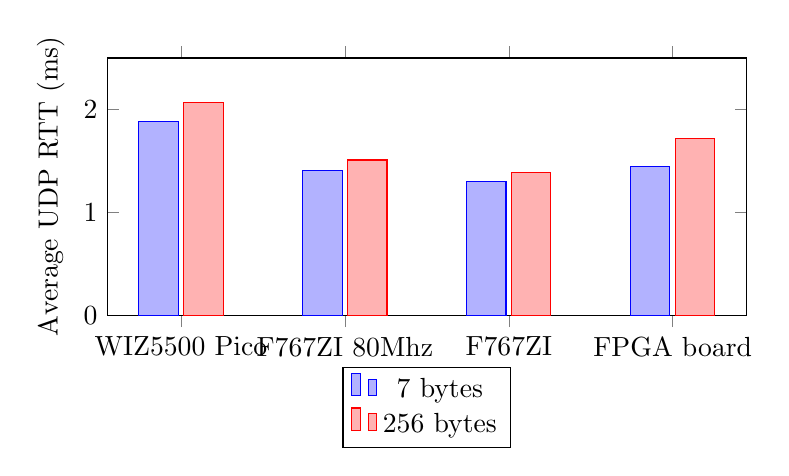
\begin{tikzpicture}
    \begin{axis}[
        ybar,
        symbolic x coords={WIZ5500 Pico, F767ZI 80Mhz, F767ZI, FPGA board},
        xtick=data,
        ylabel={Average UDP RTT (ms)},
        legend style={at={(0.5,-0.2)},anchor=north},
        enlarge x limits=0.15,
        ymin=0,
        ymax=2.5,
        width=0.8\textwidth,
        height=0.4\textwidth,
        bar width=0.5cm
    ]
    \addplot coordinates {
        (WIZ5500 Pico,1.88)
        (F767ZI 80Mhz,1.41)
        (F767ZI,1.30)
        (FPGA board,1.45)
    };
    \addplot coordinates {
        (WIZ5500 Pico,2.07)
        (F767ZI 80Mhz,1.51)
        (F767ZI,1.39)
        (FPGA board,1.72)
    };
    \legend{7 bytes,256 bytes}
    \end{axis}
    \end{tikzpicture}
    \caption{Average UDP RTT for different devices and payload sizes.}
    \end{figure}
    

Testing with WIZ5500 Pico, avg udp rtt was 1.88ms from 1000 tests with a payload of 7 bytes.
Testing with WIZ5500 Pico, avg udp rtt was 2.07ms from 1000 tests with a payload of 256 bytes.

Testing with LwIP Nucleo-F767ZI at 80Mhz, avg udp rtt was 1.41ms from 1000 tests with a payload of 7 bytes.
Testing with LwIP Nucleo-F767ZI at 80Mhz, avg udp rtt was 1.51ms from 1000 tests with a payload of 256 bytes.

Testing with LwIP Nucleo-F767ZI, avg udp rtt was 1.30ms from 1000 tests with a payload of 7 bytes.
Testing with LwIP Nucleo-F767ZI, avg udp rtt was 1.39ms from 1000 tests with a payload of 256 bytes.


Testing with FPGA board, avg udp rtt was 1.45ms from 1000 tests with a payload of 7 bytes.
Testing with FPGA board, avg udp rtt was 1.72ms from 1000 tests with a payload of 256 bytes.


\subsection{Firewall performance}

The hardware packet filter in this design has previously be found to induce a 4.48us delay and does not change the throughput of the device. 

A software based implementation of the firewall was created on the Nucleo-F767ZI board. Also with 8 rules. After measuring with an with an oscilloscope for the time it takes to compute whether or not to forward the packet, the timings depended on first how many rules there are, where a valid rule is matched (start or end of the sequence), if there is like terms between invalid rules and so on. 

As a best case, the time was found to be 3.14us (figure \ref{fig:sw_pf_best_case}) while an average-to-bad case was 10.76us (figure \ref{fig:sw_pf_bad_case}).



\begin{figure}[h]
    \centering
    \begin{subfigure}[b]{0.45\textwidth} % Adjust the width to your needs
        \includegraphics[width=\textwidth]{Images/sw_pf_best_case.png}
        \caption{Best case scenario}
        \label{fig:sw_pf_best_case}
    \end{subfigure}
    \hfill % this will add a small space between the two images
    \begin{subfigure}[b]{0.45\textwidth} % Adjust the width to your needs
        \includegraphics[width=\textwidth]{Images/sw_pf_bad_case.png}
        \caption{Average case}
        \label{fig:sw_pf_bad_case}
    \end{subfigure}
    \caption{Software packet classifier timings}
    \label{fig:sw_pf_timings}
\end{figure}

Importantly these delays unlike the FPGA one, do impact throughput as the processor is limited to filtering the packets and not doing other things like recieving another packet. 

\subsection{Thermal analysis}

A thermal camera was used to record the temperatures periodically. At an ambient room temperature of $24.8\degree C$ throughout the test, after 5mins the WIZ5500 ethernet chip heated to $58.0\degree C$ and RP2040 was at $46.6\degree C$. While the FPGA was at $38.0 \degree C$. This is a bit of an unfair comparison as the physical size of the FPGA is much larger than the WIZ5500. After two hours of constant UDP ping requests to both devices, figure \ref{fig:thermal_2hr_fpga_pico} shows the FPGA board and WIZ5500 board's temperature gradient. The FPGA plateaued to a maximum of $40.4 \degree C$ while the WIZ5500 was $1.c \degree C$ cooler at, $56.8 \degree C$. This could be due to accuracy of the measurements, in addition to not getting aiming the thermal camera in the hottest part. The RP2040 chip however was measured to be $53.2 \degree C$. Some additional thermal images can be found in the appendix. 



\begin{figure}[h]
    \centering
    \begin{subfigure}[b]{0.45\textwidth} % Adjust the width to your needs
        \includegraphics[width=\textwidth]{Images/flir_2hs.jpg}
        \caption{FPGA board (top) and WIZ5500 Pico (bottom)}
        \label{fig:thermal_2hr_fpga_pico}
    \end{subfigure}
    \hfill % this will add a small space between the two images
    \begin{subfigure}[b]{0.45\textwidth} % Adjust the width to your needs
        \includegraphics[width=\textwidth]{Images/flir_nucleo_milkv.jpg}
        \caption{Nucleo board (left) and MilkV Duo (right)}
        \label{fig:thermal_2hr_nucleo_milkv}
    \end{subfigure}
    \caption{Thermal images of boards under test after two hours}
    \label{fig:thermal_2hr}
\end{figure}

A STM32 Nucleo-F767ZI board and a MilkV Duo board was also tested (figure \ref{fig:thermal_2hr_nucleo_milkv}). After two hours, the STM32F767 reached a temperature of $36.8\degree C$ while the LAN8742 reached $36.2\degree C$. The MilkV Duo which consists of the Ethernet PHY internally reached $38.1\degree C$ after two hours.

These temperatures though cannot be considered as accurate, but rather used as an indication to see the hotspots in the boards and determine if one board gets excessively hot over the other. With this in mind, The WIZ5500 seems to reach the hottest out of the boards tested. The FPGA itself was consistently the lowest temperature across the board with the MilkV coming in a close second (considering it only has one source of heat).


\subsection{Power consumed between boards}

\begin{figure}[ht]
    \centering
    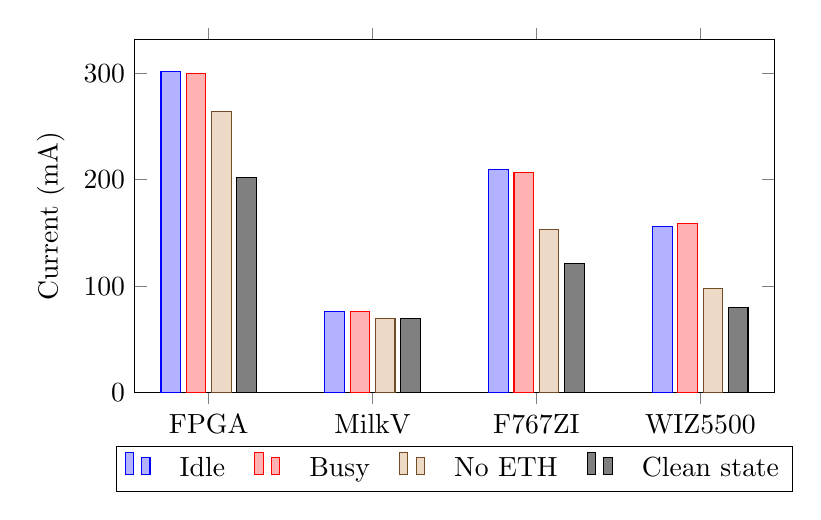
\begin{tikzpicture}
        \begin{axis}[
            ybar,
            bar width=0.25cm,
            width=0.8\textwidth,
            height=0.5\textwidth,
            enlarge x limits=0.15, % Adjusted value to make the bars closer
            ylabel={Current (mA)},
            symbolic x coords={FPGA, MilkV, F767ZI, WIZ5500},
            xtick=data,
            legend style={
                at={(0.5,-0.15)},
                anchor=north,
                legend columns=-1,
                legend cell align=left,
                legend image post style={scale=1}, % Adjust this value for spacing
                column sep=0.3cm % Adjust the space between each legend entry
            },
            legend cell align=left,
            ymin=0,
        ]
        \addplot coordinates {
            (FPGA, 301.4)
            (MilkV, 76.27)
            (F767ZI, 209.25)
            (WIZ5500, 155.88)
        };
        \addlegendentry{Idle}
        
        \addplot coordinates {
            (FPGA, 300.13)
            (MilkV, 76.53)
            (F767ZI, 206.9)
            (WIZ5500, 158.67)
        };
        \addlegendentry{Busy}
    
        \addplot coordinates {
            (FPGA, 264)
            (MilkV, 69.23)
            (F767ZI, 153.46)
            (WIZ5500, 97.9)
        };
        \addlegendentry{No ETH}

        % New data for "Complete Idle"
        \addplot coordinates {
            (FPGA, 202.13)
            (MilkV, 69.23)
            (F767ZI, 121.31)
            (WIZ5500, 80.35)
        };
        \addlegendentry{Clean state}

        \end{axis}
    \end{tikzpicture}
    \caption{Comparison of Idle, Busy, and No eth currents for devices}
    \label{fig:power_comparison}
    \end{figure}
    


In Appendix \ref{app:current_measurements} figure \ref{tab:power_consumption} shows the same data in table form presenting numerical values.

From figure \ref{fig:power_comparison}, the difference between the clean state and the busy states can be learned. The FPGA board had the largest difference at 99.27mA, compared to the 87.94mA difference witnessed in the F767ZI board. What must be taken into consideration is that the measurement for the FPGA board is without the hardware design (both Ethernet MAC, packet filter and RISC-V core) applied. Another reading of 283.75mA was observed when the design and hardware had been loaded (no firmware). What this means is that even though the FPGA board has the highest quiescent current amoungst the devices, it still has the larger design current for the project itself. 

The smaller difference from the no Ethernet attached to the active state on the FPGA in comparison to the differences noticed on the F767ZI and WIZ5500 boards indicates that this is likely due to the MAC hardware in the F767ZI and WIZ5500 enters a sleep state to consume less current. The hardware designed in this thesis did not take this case into consideration. 


\subsection{Security analysis}
Only the FPGA board designed in this thesis has a hardware packet filter. The other devices need to implement a software based packet filter. On the surface this makes the two sound equivalent. However, software based firewalls may be susceptible to power-glitch attacks. Power glitch attacks are a common vulnerability in embedded systems. It consists of switching off and on power very rapidly at a critical point in the code to essentially bypass a certain instruction. While this is highly unlikely and often hard to implement, it is an advantage nonetheless.  

As the packet filter is designed in hardware and is directly reading the bits from the PHY and doesn't consist of instructions as such, the hardware packet classifier in this design should not susceptible to a power glitch attack. Formal testing of this however was not part of the scope of this thesis.


\section{Power analysis}

\subsection{Theoretical analysis }

Vivado provides a post synthesis power analysis summary for the design. While these are depenant on a lot of variables, they should provide a basis as to what to expect and help with optimisation of power within the design. The design was observed to take a total of 0.487W (figure \ref{fig:post_synth_power_summary}) where 0.383W of that is dynamic and depends on the operations taking place. 

\begin{figure}[h]
    \centering
    \includegraphics[width=0.75\textwidth]{Images/power_summary.png}
    \caption[Post synthesis power summary for design]{Post synthesis power summary for design.}
    \label{fig:post_synth_power_summary}
\end{figure}


Vivado further breaks down the design into the different hierarchical components shown in table \ref{tab:power_consumption}. Notably most of the power consumption in the design is a result of the RISC-V processor in the design. Notably the Ethernet hardware and packet filter consumes under 100mW. 

\begin{table}
    \centering
    \caption{Power consumption of components.}
    \begin{tabular}{|l|c|}
        \hline
        \textbf{Name} & \textbf{Total (W)} \\
        \hline
        neorv32 & 0.158 \\
        clk control & 0.097 \\
        ethernet\_mac & 0.097 \\
        packet classifier & 0.002 \\
        \hline
    \end{tabular}
    \label{tab:power_consumption}
\end{table}




\subsection{Measured analysis}

As the voltage would remain constant between devices (all powered over USB), only the current was measured. These results however should be taken with caution as they do not account for regulator inefficiencies and do not give a true current reading of the device, rather just an indication. 


The device for testing the current was the Nordic Semiconductor Power Profiler Kit 2 which can record at up to 100kSa/s. For the tests in this report, only a sampling rate of 10kSa/s was used as it produces less noisy results. 

As a baseline, the Nexys A7 board draws 200mA (1W at 5V) with no design applied and is due to all the additional components on the board. With the design loaded up but without the processor flashed, the board took 284.4mA. After flashing the board, the idle current reached an average of 301.84mA. Multiplying this by 5V gives us a power draw of 1.51W. To factor in the quiescent current for the other devices on the FPGA board and if it is assumed that the 200mA reading solely for the other components on the FPGA board, it can be found that the design draws around 0.51W. This is rather close to what the synthesis tool calculated. 

A series of tests were then done and the currents were measured. By pinging the device every 50ms, the average current consumption was 300.72mA. Interestingly, the current consumption was cyclic similar to what is shown in figure \ref{fig:ppk_icmp_ping}. A UDP ping test was conducted and had an average current draw of 301.13mA. In both the ICMP and UDP pings, the current consumption was of similar style where the variance of the current was about 10mA. 


If the packets are now blocked by the filter, more about the design in terms of power consumption can be learned. After adding a rule in the packet filter, very little could be observed in the current consumption over the unblocked case. The same cyclic pattern in figure \ref{fig:ppk_icmp_ping} could be seen. An average of 300.92mA was been consumed by the device and is within the margin of error of the device. Figure \ref{fig:ppk_icmp_ping} shows the that the period for the current waveform is about 83ms, which is much larger than the 50ms between pings to the device. After filming the status LED on the PHY output at 240 frames per second, the period of the LED was 20 frames equivalent to $\approx 84ms$ which aligns with the current measurements. 


\begin{figure}[h]
    \centering
    \includegraphics[width=0.9\textwidth]{Images/PPK_ping_zoom.png}
    \caption[Zoomed in current consumption for ICMP pings]{Zoomed in current consumption for ICMP pings.}
    \label{fig:ppk_icmp_ping}
\end{figure}



The next test was done when accessing the webserver. Figure \ref{fig:ppk_http_annotated} shows 5 different regions where each region is a result of a different action. The left most tests is from the inital HTTP requests to get the index page. Notably, there is 2 separate sections here, this is because the client fetches the html, css and favicon first and then requests the main (and much larger) javascript file after. The readings for each of these points is given as: average current, maximum current and time going from top to bottom. 

The second test is what happens when you click to navigate to the about page. The third event is when navigating to the config page and the 4th event is what happens when you press the 'load rules' button. The final test case is a refresh on the main page for the statistics. Notably, as the javascript (thus client) is doing the routing and page handling, future requests to get the contents of the pages are not needed, but only small API requests to update the data. Coincidentally, these first 3 requests also trigger a SD card read and explains the higher current draw. The fourth request also creates a read request to the SD card, but only needs to read a single page. The fifth request does not involve a read or write to the SD card, but rather just a simple SPI transaction takes place and consequently doesn't draw much additional power. 

\begin{figure}[h]
    \centering
    \includegraphics[width=0.9\textwidth]{Images/PPK_http_annotated.png}
    \caption[Current consumption of FPGA board with HTTP requests]{Current consumption of FPGA board with HTTP requests.}
    \label{fig:ppk_http_annotated}
\end{figure}



% HOW TO ADD ADDITIONAL CHAPTERS
% Step One: Add a new folder called "ChapterX" (X being the chapter number).
% Step Two: Within the folder add a new .tex file by clicking the "New File" button in the Overleaf Menu. Rename the file to a title of your choice.
% Step Three: Copy the Chapter 2 headline and "\input" command located above and insert it below Chapter 2.
% Step Four: Rename the headline to your specific chapter number, change the input command to include the name of the folder you created and the name of the file you created.
% Repeat this process for every chapter.

%CONCLUSION CHAPTER
\chapter[Conclusion]{Conclusion}
\label{Chap:Conclusion}

\section{Summary}

This thesis explored the design and implementation of a hardware packet filter, Ethernet MAC with a RISC-V softcore processor. The Ethernet MAC and packet filter were created from scratch, while the NEORV32 RISC-V softcore was used to interface with the custom hardware. This was all implemented on a Xilinx Artix 7 FPGA board with the LAN8720A PHY. The design was evaluated and compared against similar preexisting solutions on the market. While the design in this thesis did not outperform the preexisting solutions in all cases, it was comparable and did provide new and unique features not seen before in the embedded systems space. In addition to the hardware, a webserver and web application was created to allow for easy configuration of the packet filter. 

The design in this thesis shows that hardware packet filters in embedded systems are feasible and consume minimal resources while providing great performance. The design was able to achieve a latency of $4\mu s$ while only consuming 571 slice LUTs and 1145 slice registers. The packet filter design was also able to achieve a power consumption of just 2mW.



\section{Limitations}
While this thesis explored the design and implementation of a hardware packet filter, Ethernet MAC with a RISC-V softcore processor, there are some limitations to the design and the research conducted. These can be summarised in the following points:


\begin{itemize}
    \item The current system only supports filtering network packets in one direction as it assumes all packets leaving the device is safe. 
    \item The design only considers IPv4 packets without IEEE 802.1Q VLAN tagging.
    \item The transmit logic is not optimised for resource usage and can be improved.
    \item Only one interface is supported due to the bandwidth limitations of the PMOD ports on the Nexys A7 board.
    \item Only HTTP and other unencrypted protocols are supported.
    \item The current design is bottlenecked from the processor - NEORV32
\end{itemize}


In addition, only one interface is supported due to the Nexys A7 board only consisting of one ethernet PHY and the additional PMOD ports are not suitable for Ethernet. This is because the PMOD ports are only rated for a 25Mhz bandwidth, while the RMII signals are 50Mhz. As such, signal integrity issues arose (see appendix \ref{app:eye_diagrams} for eye diagram) and restricted the use to just one interface - the onboard PHY. A new development board with two PHYs would be needed.











\section{Sustainability}



The sustainability of the designed system in this thesis is multi-layered with considerations in hardware, software, and web development taken into consideration. 

Starting at the hardware level, the specific implementation in this thesis uses the Digilent Nexys A7 FPGA board with a Xilinx Artix 7 FPGA and a LAN8720A PHY. The LAN8720A PHY uses the standardised RMII interface, increasing the portability across various FPGAs assuming adequate resources. Likewise, other RMII PHY chips could be swapped out with the LAN8720A without issue due to the standardised interfae. The specific implementation of the hardware in this thesis requires minimal modification to support other media independent interfaces such as RGMII or XGMII. The main difference would be in the input and output FIFOs being able to support the different clock rates and bit widths. Apart from the clocking IP block, the design is written in vendor-agnostic VHDL and can be easily ported to other FPGAs. 

The TCP/IP standards including the IEEE 802.3 Ethernet standards and protocols such as IP, TCP, and UDP, have being around for decades with minimal adjustments to the standards since their inception. New features in these standards typically are additive and do not modify the packet structure itself, allowing for backwards compatibility. An example of this is the introduction of IPv6 in 1998 \cite{rfc2460}. This is important when designing a hardware layer packet filter which assumes the bit positioning of the fields in the packet. Considering this, the packet filter should be still applicable in the future as the packet structure is unlikely to change.


The choice of using a RISC-V processor architecture is another sustainable consideration made in this project. While RISC-V is royalty-free and the core instruction set architecture is open-source, not all implementations of RISC-V cores are open-source or free. The specific implementation of RISC-V used in this thesis is the NEORV32, which is open-source and free to use under the BSD-3-Clause license \footnote[1]{See: https://github.com/stnolting/neorv32/blob/main/LICENSE}. This importantly allows for commercial use and redistribution, but does not carry any liability. Additionally, the NEORV32 is still in active development and is continually getting updated with new features and bug fixes. While this means that new features and security patches will get added, it also incurs additional work to update the design to the latest version. The future of the open-source design is also vulnerable to becoming abandoned if the developer decides to stop working on it. 


Similarly to the NEORV32, FreeRTOS and their first-party FreeRTOS-Plus-TCP library are also open-source and free to use under the MIT license \footnote[2]{See: https://www.freertos.org/a00114.html}. Like the NEORV32, FreeRTOS and it's libraries are actively maintained by Amazon and feature updates, albeit less frequently than the NEORV32. The FreeRTOS-Plus-TCP library is also feature-rich and is continually getting updated, however, it's documentation and community support is more limited than that of LwIP.



In terms of web development, Vue.js was used as a framework for web development. Primary issues of concern for web applications are dependencies and library support and maintenance. In this project, only a small handful of packages were used, each of which are well maintained and have a large community support. If future designs were to use Vue.js with other packages, it is recommended that the packages used are well maintained. Like the TCP/IP stack, HTTP, HTML, Javascript and CSS, which Vue.js is built upon, are heavily standardised but do change over time. As such, future designs should be aware of these changes and adapt accordingly.


Finally, the security of the design poses the greatest risk to sustainability. Malicious bad actors are continually innovating and finding new ways to breach systems. Despite this, the core design of the packet filter remains fundamentally strong due to it's basic filtering capabilities. While it will not prevent all cyber attacks, it can be used as a tool in a much larger system to help mitigate the risk of such attacks. Further fortifications can be made to the system architecture by using HTTPs, public key cryptography, and deep packet inspection.





\section{Recommendations and future work}

In light of the findings in this thesis, several key recommendations can be made for future work in the area of embedded system SoC design which features Ethernet connectivity.

The primary recommendation is to incorporate dedicated hardware packet filtering into SoC designs. As demonstrated in this thesis, the resource utilisation for the packet filtering logic is minimal (571 slice LUTs and 1145 slice registers) and can be easily integrated into the design with minimal impact to cost. Superior latency, throughput and power consumption metrics are only some of the benefits presented in this thesis over the conventional software based packet filters. Additionally, the potential resilience against potential security vulnerabilities is another key advantage of this approach.

While the NEORV32 is a solid general-purpose softcore processor, it seemed to bottleneck the design and witheld the design from achieving better performance. The CVITEK CV1800B, used in the MilkV-Duo and compared in this thesis, is a powerful SoC with an abundance of resources including a hardware MAC and PHY, but falls short of including a hardware packet filter. An ideal choice would be to have the performance of the CVITEK CV1800B with the hardware packet filtering capabilities of the design presented in this thesis. This would give the best of both worlds, performance and security.

Alternatively, research into using hybrid SoC FPGAs such as the Xilinx Zynq lineup which include an FPGA and a hardcore processor connected over a high speed fabric could be a good avenue. This provides the flexibility of an FPGA with the performance of a hardcore processor, ideal for small scale designs that would otherwise be too expensive for custom silicon.

Leveraging single page application frameworks such as Vue.js for use in embedded systems is another recommendation resulting from the work done in this thesis. Light-weight applications and low power devices can benefit greatly from the use of such frameworks as fewer network traffic is required due to client-side routing and static web content. In combination with a lightweight API, dynamic data can be obtained with minimal network traffic, making the user experience seamless and responsive.

In addition to these recommendations for future designs, the work in this thesis can be extended in the following areas:

\begin{itemize}
    \item Redesign of the transmit logic to consume less resources while not losing on speed/performance, 
    \item Add a second Ethernet interface to filter traffic for other devices on the network, 
    \item Utilise the DDR2 RAM to free up BRAM in the FPGA, 
    \item Implement public key cryptography for HTTPS,
    \item Support faster media interfaces, eg RGMII for 1Gbit/s or XGMII for 10Gbit/s,
    \item Use a different bus interconnect for the processor, eg AXI4, and
    \item Look into using LwIP over FreeRTOS-Plus-TCP.
\end{itemize}






% ***************************************************
% Bibliography
%****************************************************
%CHOOSE YOUR BIB STYLE AND FILE.
%We have included the following two referencing styles for you to use in your thesis. You can add an alternate style if you prefer.

%Style: apalike = this is an (Author, Year) referencing style similar to APA
%Style: elsarticle-num = this is a numbered referencing style that will display the bibliography in citation order

%To use one of the styles provided ensure the % is removed from the start of the line, and the other option is commented out with a % at the start of the line. The style elsarticle-num is active by default.

%\bibliographystyle{apalike}
\bibliographystyle{ieeetr}

\bibliography{./References/Bibliography}


%When you have finished your thesis we recommend that you manually fix any errors in your bibliography. 
%To do this, compile, copy the .bbl into a new .tex file and include this here after commenting out the other bibliography commands. Make corrections in that .tex file.

% ***************************************************
% Appendices
%**************************************************** 
%UNCOMMENT THIS SECTION IF YOU ARE USING APPENDICES.
%Simply adapt the same formatting used for other chapters.
\appendix
% If you need appendix in your thesis then consider the following appendix file (you can add more if you need more) otherwise you should not consider it in your main thesis.
% ***************************************************
% Appendix
% ***************************************************
\chapter{Appendix}

Write your appendix here. Following two are examples. 


\section{Neorv32 memory address space layout}
\label{app:mem_address}
\begin{figure}[h!]
    \centering
    \includegraphics[width=1\textwidth]{Images/neorv32_address_space.png}
    \caption{Neorv32 Memory Address space.}
\end{figure}



\section{FPGA primitives utilisation}
\label{app:res_usage}
\begin{table}
    \centering
    \caption{FPGA primitives utilisation for XC7A100T}
    \begin{tabular}{|l|r|l|}
        \toprule
        Ref Name   & Used & Functional Category \\
        \midrule
        LUT6       & 16262 & LUT \\
        LUT5       & 14820 & LUT \\
        FDRE       & 14500 & Flop \& Latch \\
        LUT3       & 13222 & LUT \\
        MUXF7      &  2436 & MuxFx \\
        FDCE       &  1875 & Flop \& Latch \\
        RAMD64E    &  1836 & Distributed Memory \\
        LUT4       &  1294 & LUT \\
        LUT2       &  1016 & LUT \\
        MUXF8      &   884 & MuxFx \\
        CARRY4     &   437 & CarryLogic \\
        LUT1       &   156 & LUT \\
        RAMB36E1   &   130 & Block Memory \\
        FDPE       &    41 & Flop \& Latch \\
        OBUF       &    40 & IO \\
        LDCE       &    36 & Flop \& Latch \\
        IBUF       &    24 & IO \\
        SRLC32E    &    21 & Distributed Memory \\
        OBUFT      &    11 & IO \\
        BUFG       &     8 & Clock \\
        FDSE       &     5 & Flop \& Latch \\
        DSP48E1    &     4 & Block Arithmetic \\
        SRL16E     &     1 & Distributed Memory \\
        MMCME2\_ADV &    1 & Clock \\
        \bottomrule
    \end{tabular}
\end{table}

\begin{table}
    \centering
    \caption{Memory Utilisation}
    \begin{tabular}{|l|r|r|r|r|r|}
        \toprule
        Site Type      & Used & Fixed & Prohibited & Available & Util\% \\
        \midrule
        Block RAM Tile &  130 &     0 &          0 &       135 & 96.30 \\
        RAMB36/FIFO*   &  130 &     0 &          0 &       135 & 96.30 \\
        RAMB36E1 only  &  130 &     - &          - &         - &    -  \\
        RAMB18         &    0 &     0 &          0 &       270 &  0.00 \\
        \bottomrule
    \end{tabular}
\end{table}

\begin{table}
    \centering
    \caption{Slice Logic Utilisation}
    \begin{tabular}{|l|r|r|r|r|r|}
        \toprule
        Site Type                 & Used & Fixed & Prohibited & Available & Util\% \\
        \midrule
        Slice LUTs*               & 40920 &     0 &          0 &     63400 & 64.54 \\
        LUT as Logic              & 39062 &     0 &          0 &     63400 & 61.61 \\
        LUT as Memory             &  1858 &     0 &          0 &     19000 &  9.78 \\
        LUT as Distributed RAM    &  1836 &     - &          - &         - &    -  \\
        LUT as Shift Register     &    22 &     - &          - &         - &    -  \\
        Slice Registers           & 16457 &     0 &          0 &    126800 & 12.98 \\
        Register as Flip Flop     & 16421 &     0 &          0 &    126800 & 12.95 \\
        Register as Latch         &    36 &     0 &          0 &    126800 &  0.03 \\
        F7 Muxes                  &  2436 &     0 &          0 &     31700 &  7.68 \\
        F8 Muxes                  &   884 &     0 &          0 &     15850 &  5.58 \\
        \bottomrule
    \end{tabular}
\end{table}


\section{Additional webpages built into the webserver.}
\label{app:additional_webpages}
\begin{figure}[h!]
    \centering
    \includegraphics[width=1\textwidth]{Images/webapp_about.png}
    \caption{Screenshot of the about page in the webapp.}
    \label{fig:web_app_about}
\end{figure}

\begin{figure}[h!]
    \centering
    \includegraphics[width=1\textwidth]{Images/webapp_config.png}
    \caption{Screenshot of the config page in the webapp.}
    \label{fig:web_app_config}
\end{figure}


\section{UDP ping times between boards}
\label{app:udp_ping_measurements}
\begin{table}[ht]
    \centering
    \caption{Average UDP RTT for different devices and payload sizes.}
    \begin{tabular}{lcc}
    \toprule
    Device & 7 bytes (ms) & 256 bytes (ms) \\
    \midrule
    WIZ5500 Pico & 1.88 & 2.07 \\
    F767ZI & 1.30 & 1.39 \\
    F767ZI 80Mhz & 1.41 & 1.51 \\
    MilkV & 1.04 & 1.09 \\
    FPGA board & 1.45 & 1.72 \\
    \bottomrule
    \end{tabular}
    \end{table}

\section{Current measurments from boards}
\label{app:current_measurements}

Table \ref{tab:power_consumption} shows the current measurments. Notably Diff1 is the difference between the Idle and No ETH fields while Diff2 is the difference between the Idle and Clean states.

\begin{table}[ht]
    \centering
    \caption{Device power consumption data (all values in mA)}
    \label{tab:power_consumption}
    \begin{tabular}{lccccccc}
    \toprule
    Device    & Idle  & Busy  & Average  & No ETH  & Clean  & Diff1  & Diff2 \\
    \midrule
    FPGA      & 301.4     & 300.13    & 300.765      & 264         & 202.13           & 37.4     & 99.27       \\
    MilkV     & 76.27     & 76.53     & 76.4         & 69.23       & 69.23            & 7.04     & 7.04       \\
    F767ZI    & 209.25    & 206.9     & 208.075      & 153.46      & 121.31           & 55.79    & 87.94       \\
    WIZ5500   & 155.88    & 158.67    & 157.275      & 97.9        & 80.35            & 57.98    & 75.53       \\
    \bottomrule
    \end{tabular}
\end{table}


\section{Thermal measurements for boards}

\begin{table}[ht]
    \centering
    \caption{Device measurements over time using FLIR One thermal camera}
    \label{tab:measurements}
    \begin{tabular}{lcccccc}
    \toprule
    Device & 5min & 10min & 30min & 1h & 2h \\
    \midrule
    FPGA & 38 & 38.2 & 38.9 & 39.1 & 40.4 \\
    MilkV & 36.7 & 39.8 & 35.5 & 39.1 & 38.1 \\
    F767ZI (STM) & 35.9 & 38.9 & 35.8 & 37.5 & 36.8 \\
    F767ZI (PHY) & 38 & 38.8 & 35.2 & 37.2 & 36.2 \\
    WIZ5500 (RP2040) & 46.6 & 53.1 & 54.6 & 54.5 & 53.2 \\
    WIZ5500 (PHY) & 58 & 59 & 58.4 & 58.5 & 56.8 \\
    \bottomrule
\end{tabular}
\end{table}



% ***************************************************
% Back Matter
%**************************************************** 
%COMMENT OUT IF YOU DO NOT WISH TO INCLUDE BACK MATTER.
% \input{./PreliminaryAndBackPages/Back.tex}

\end{document}
